% !TEX root = ../main.tex

\section{Introduction}
\begin{frame}{\insertsec}
	\begin{itemize}
    \item Nowadays Machine Learning is widely used
    \item Medical images can be obtained using MRI, PET or CT scans but are underused
    \item Different methods have appeared to analyze these data for image classification,
    object detection, segmentation...
    \item Deep learning models aim to be able to unlock the full potential of medical imaging
    \item Hand-crafted radiomic features can be extracted from medical images
  \end{itemize}
\end{frame}

\subsection{Survival Analysis}
\begin{frame}{\insertsubsec}
  Survival analysis models usually have:
  \begin{itemize}
    \item Baseline data \( x \)
    \item Event \( E \in \{0, 1\} \)
    \item Time \( T \)
  \end{itemize}
  
  Survival function:
  \[
    S(t) = \Pr(T \ge t)
  \]

  Hazard function:
  \[
    \lambda(t) = \lim_{\Delta t \rightarrow 0}
    \frac{\Pr(t \le T < t + \Delta t | T \ge t)}{\Delta t}
  \]
\end{frame}

\begin{frame}

  Casting the survival problem as a ranking is a way of dealing with censored data.

  \begin{columns}
    \begin{column}{.5\textwidth}
      \begin{figure}
        \centering
        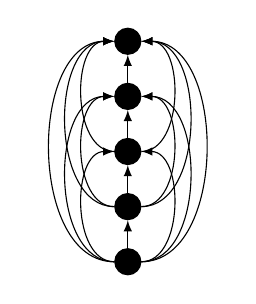
\begin{tikzpicture}[scale=.7]
  \tikzstyle{bDot}=[circle, fill=black, draw]
  \foreach \y in {1,...,5} {
    \node[bDot] (D-\y) at (0, \y) {};
  }

  \foreach \y in {1,...,4} {
    \pgfmathsetmacro{\z}{int(\y + 1)}
    \draw[-latex] (D-\y) -- ({D-\z}.south);
  }

  \foreach \y in {1,...,3} {
    \pgfmathsetmacro{\z}{int(\y + 2)}
    \foreach \j in {\z,...,5} {
      \ifthenelse{\y=2 \OR \y=3}{
        \draw[-latex] (D-\y) to[bend left=90] (D-\j);
      }{
        \draw[-latex] (D-\y) to[bend right=90] (D-\j);
      }
    }
  }
\end{tikzpicture}

        \caption{Uncensored data}
      \end{figure}
    \end{column}
    \begin{column}{.5\textwidth}
      \begin{figure}
        \centering
        \begin{tikzpicture}
  \foreach \y in {1,...,5} {
    \ifthenelse{\y=2 \OR \y=4}{
      \node [circle, fill=white, draw=black] (D-\y) at (0, \y) {};
    }{
      \node [circle, fill=black, draw=black] (D-\y) at (0, \y) {};
    }

    \foreach \y in {3,4,5} {
      \draw [-latex] (D-1) to[bend right=90] (D-\y);
    }

    \foreach \y/\z in {1/2, 3/4} {
      \draw [-latex] (D-\y) -- (D-\z);
    }
    \draw [-latex] (D-3) to[bend left=90] (D-5);
  }
\end{tikzpicture}

        \caption{Censored data}
      \end{figure}
    \end{column}
  \end{columns}
\end{frame}

\begin{frame}
  \begin{itemize}
    \item Both of them are uncensored (\( \bm{E}_i = \bm{E}_j = 1\))
    \item The uncensored time of one is smaller than the censored survival time of the other
    (\( \bm{T}_i < \bm{T}_j | \bm{E}_i = 1; \bm{E}_j = 0 \))
  \end{itemize}

  Concordance Index:
  \[
    CI = \frac{\text{Good predictions}}{\text{Total predictions}} \in [0, 1]
  \]
\end{frame}
